\documentclass[10pt,aspectratio=169, colorlinks=true, linkcolor=circlBlue]{beamer}

% tlp allowed values: clear, green, amber, amber+strict, red
\usetheme[numbering=fraction, progressbar=frametitle]{circl}

% for code highlighting
\usepackage{minted}
% to draw pingus
\usepackage{tikzpingus}
% to draw boxes to catch attention
\usepackage{awesomebox}
% For hyperlinks in the document and PDF metadata
\usepackage{hyperref}
% useful only if we want to customize minted background
\usepackage{tcolorbox}

\usepackage{multicol}

\usepackage{appendixnumberbeamer}
\usepackage{xcolor}
\usepackage{etoolbox}
\usepackage{tikz}
\usetikzlibrary{
    positioning,
    fit,
    arrows.meta
}

% ---------------------------------------------------------
% Colors
% ---------------------------------------------------------

\definecolor{phaseactive}{RGB}{220,220,220}
\definecolor{phaseinactive}{RGB}{90,90,90}
\definecolor{circlRed}{HTML}{EE2338}

%
% compile with -shell-escape in order to use minted
% $ pdflatex  -interaction=nonstopmode -shell-escape presentation.tex
%


\hypersetup{
    pdftitle={MISP Introduction},    % Title
    pdfauthor={Sami Mokaddem, David Cruciani},               % Author
    pdfsubject={Introduction and recent new features}, % Subject
    pdfkeywords={MISP, CTI, Threat Intelligence}, % Keywords
    colorlinks=false,                       % Color links instead of boxes
    linkcolor=blue,                        % Color of internal links
    citecolor=blue,                        % Color of citations
    urlcolor=blue                          % Color of external links
}

% set the logo to put in the title page
\titlegraphic{\noindent\hfill
\includegraphics[width=0.25\textwidth]{img/logo-circl.pdf}}
\title{MISP Introduction and recent new features}
\subtitle{CIRCL - 2026}
\date{\today}
\author{}
\institute{MISP Project \normalurl{https://misp-project.org}}
% if set inserts a title link into the title page
\titlelink{\faHome\space \normalurl{https://www.misp-project.org}}

\begin{document}

% include custom commands

% Place here your custom commands, it will be included in presentation.tex

\newcommand{\normalurl}[1]{\href{#1}{#1}}

\newcommand{\footnoteurl}[1]{\footnote{\scriptsize\url{#1}}}

\newcommand{\rocketbox}[1]{%
	\awesomebox[circlRed]{1pt}{\faRocket}{circlBlue}{#1}%
}


% =========================================================
% STORY STATUS FOOTER
% =========================================================
%
% Usage:
%
% 1. Put this in your preamble
%
% 2. Before each section, define the current phase:
%
%    \storyphase{Incident}
%    \storyphase{Correlation}
%    \storyphase{Monitoring}
%    \storyphase{Operations}
%    \storyphase{Governance}
%
% 3. The footer automatically highlights the current phase
%
% =========================================================

% ---------------------------------------------------------
% Current phase holder
% ---------------------------------------------------------

\definecolor{phaseactive}{RGB}{255,255,255}
\definecolor{phaseinactive}{RGB}{220,220,220}

\newcommand{\currentstoryphase}{}
\newcommand{\allstoryphases}{}

\newcommand{\storyphase}[1]{%
    \gdef\currentstoryphase{#1}%
    \hypertarget{#1}{}
}

\newcommand{\setphases}[1]{%
    \gdef\allstoryphases{#1}%
}

\newcommand{\phasetag}[1]{%
    \expandafter\ifstrequal\expandafter{\currentstoryphase}{#1}
        {\color{phaseactive}\textbf{\scriptsize \hyperlink{#1}{#1}}}
        {\color{phaseinactive}\hyperlink{#1}{#1}}%
}

% ---------------------------------------------------------
% Render one phase
% ---------------------------------------------------------
% \newcommand{\phasetag}[1]{%
%     \expandafter\ifstrequal\expandafter{\currentstoryphase}{#1}
%         {\color{phaseactive}\textbf{#1}}
%         {\color{phaseinactive}#1}%
%     }


% ---------------------------------------------------------
% Render all phases
% ---------------------------------------------------------
% \newcommand{\renderphases}{%
%     \foreach \x [count=\i] in \allstoryphases {%
%         \phasetag{\x}%
%         \ifnum\i<\foreachcount
%             \hspace{1.2em}|\hspace{1.2em}%
%         \fi }%
%     }

\newif\iffirstphase

\newcommand{\renderphases}{%
    \global\firstphasetrue
    \foreach \x in \allstoryphases {%
        \iffirstphase
            \global\firstphasefalse
        \else
            \hspace{1.2em}|\hspace{1.2em}%
        \fi
        \expandafter\phasetag\expandafter{\x}%
    }%
}


% ---------------------------------------------------------
% Custom footer
% ---------------------------------------------------------

\setbeamertemplate{footline}
{
    \leavevmode%
    \begin{beamercolorbox}[
        wd=\paperwidth,
        ht=3.2ex,
        dp=1.2ex,
        leftskip=1em,
        rightskip=1em
    ]{author in head/foot}
    \tiny
    \insertframenumber{} / \inserttotalframenumber
    \hfill
    \renderphases
    \end{beamercolorbox}
}

% \setbeamertemplate{footline}
% {
%     \leavevmode%
%     \begin{beamercolorbox}[
%         wd=\paperwidth,
%         ht=3.2ex,
%         dp=1.2ex,
%         leftskip=1em,
%         rightskip=1em
%     ]{author in head/foot}
%     \tiny
%     \insertframenumber{} / \inserttotalframenumber
%     \hfill
%     \phasetag{Incident}
%     \hspace{1.2em}|\hspace{1.2em}
%     \phasetag{Correlation}
%     \hspace{1.2em}|\hspace{1.2em}
%     \phasetag{Monitoring}
%     \hspace{1.2em}|\hspace{1.2em}
%     \phasetag{Operations}
%     \hspace{1.2em}|\hspace{1.2em}
%     \phasetag{Governance}
%     \hspace{1.2em}
%     \end{beamercolorbox}
% }

% Optional: remove navigation symbols
\setbeamertemplate{navigation symbols}{}

% Nice badge.
% Usage:
% \entitytag{border-color}{fill-color}{text-label}
% \entitytag{blue!60!black}{blue!5}{Internal MISP}
\newcommand{\entitytag}[3]{%
\tikz[baseline=(X.base)]{
    \node[
        draw=#1,
        fill=#2,
        rounded corners=2pt,
        inner xsep=1.5pt,
        inner ysep=0pt
    ] (X) {\strut #3};
}}


% Create a link button in the bottom-right corner that jump to the target
% Usage:
% \jumpto{hyperlinkID}{textlabel}
\newcommand{\jumpto}[2]{%
\begin{tikzpicture}[remember picture,overlay]
    \node[anchor=south east]
        at ([yshift=10pt]current page.south east)
    {
        \hyperlink{#1}{\beamergotobutton{#2}}
    };
    \end{tikzpicture}
}
% Create a link button in the bottom-right corner that return to the target
% Usage:
% \returnto{hyperlinkID}{textlabel}
\newcommand{\returnto}[2]{%
\begin{tikzpicture}[remember picture,overlay]
    \node[anchor=south east]
        at ([yshift=0pt]current page.south east)
    {
        \hyperlink{#1}{\beamerreturnbutton{#2}}
    };
    \end{tikzpicture}
}

% =========================================================
% Bootstrap-like Alert Component
% =========================================================

% ---------------------------------------------------------
% Colors
% ---------------------------------------------------------

\definecolor{alertInfoBg}{HTML}{D1ECF1}
\definecolor{alertInfoBorder}{HTML}{7FC6D1}
\definecolor{alertInfoText}{HTML}{0C5460}

\definecolor{alertWarningBg}{HTML}{FFF3CD}
\definecolor{alertWarningBorder}{HTML}{E0C24F}
\definecolor{alertWarningText}{HTML}{856404}

\definecolor{alertDangerBg}{HTML}{F8D7DA}
\definecolor{alertDangerBorder}{HTML}{D98C95}
\definecolor{alertDangerText}{HTML}{721C24}

% ---------------------------------------------------------
% Internal style selector
% ---------------------------------------------------------

\newcommand{\alertboxsetup}[1]{%

    % INFO
    \ifstrequal{#1}{info}{
        \colorlet{alertbg}{alertInfoBg}
        \colorlet{alertborder}{alertInfoBorder}
        \colorlet{alerttext}{alertInfoText}
    }{}

    % WARNING
    \ifstrequal{#1}{warning}{
        \colorlet{alertbg}{alertWarningBg}
        \colorlet{alertborder}{alertWarningBorder}
        \colorlet{alerttext}{alertWarningText}
    }{}

    % DANGER
    \ifstrequal{#1}{danger}{
        \colorlet{alertbg}{alertDangerBg}
        \colorlet{alertborder}{alertDangerBorder}
        \colorlet{alerttext}{alertDangerText}
    }{}
}

% ---------------------------------------------------------
% Alert command
% ---------------------------------------------------------

\newcommand{\alertbox}[3]{%

    \alertboxsetup{#1}

    \begin{center}
    \begin{tikzpicture}

    \node[
        draw=alertborder,
        fill=alertbg,
        rounded corners=2pt,
        line width=0.6pt,
        inner sep=10pt,
        text width=0.92\linewidth,
        align=left
    ] {

        {\color{alerttext}\bfseries #2}

        \vspace{0.35em}

        {\color{alerttext}#3}
    };

    \end{tikzpicture}
    \end{center}
}
% =========================================================
% Generic capability card
% =========================================================

\newcommand{\card}[4]{
\begin{tikzpicture}
\node[
    draw=black!20,
    fill=black!3,
    rounded corners=3pt,
    minimum width=#1,
    minimum height=#2,
    inner sep=5pt,
    align=left
]{
    \begin{minipage}{0.9\linewidth}
        {\large #3}

        \vspace{0.3em}

        \small
        #4
    \end{minipage}
};
\end{tikzpicture}
}

% Set phases to be displayed on the footer
\setphases{ Introduction, New Features }


% Title page
\begin{frame}
	\titlepage%
\end{frame}


% =========================================================
% INTRODUCTION
% =========================================================

\nosectionpage{Introduction}
\storyphase{Introduction}

\subsection{Workshop Goals}

\begin{frame}{Workshop Overview}

\textbf{Audience}
\vspace{-0.5em}
\begin{itemize}
    \item \textbf{Primary}: Cyber Threat Intelligence Analysts
    \item \textbf{Secondary}: SOC and Incident Response Teams
    \item \textbf{Expected MISP Knowledge}: None
    \item \textbf{Training level}: Basic
\end{itemize}


\textbf{Workshop Objectives}
\vspace{-0.5em}
\begin{itemize}
    \item Understand how MISP supports \textbf{operational investigations}
    \item Transform unstructured data \textbf{actionable intelligence}
    \item \textbf{Correlate} incidents across teams and partners
    \item \textbf{Enrich} data and \textbf{Collaborate}
\end{itemize}

\end{frame}

\begin{frame}
    \frametitle{Training Agenda}

	\begin{itemize}
	    \item \textbf{Presentation of MISP} {\small (1h)}
	    \begin{itemize}
	        \item Introduction {\small (30min)}
	        \item Basic UI, Concept \& Terminology {\small (30min)}
	    \end{itemize}
	    \item \alert{\textbf{Break}} {\small (15min)}
	    \item \textbf{Demonstration and Familiarization} {\small (1h30)}
	    \begin{itemize}
	        \item \textbf{Walkthrough on encoding data} {\small (30min)}
	        \item \textbf{Faster encoding \& Enrichment} {\small (20min)}
	        \item \textbf{Getting The Most Out Of Your Data} {\small (20min)}
	        \item \textbf{Collaboration and Sharing} {\small (20min)}
	    \end{itemize}
	    \item \alert{\textbf{Lunch Break}} {\small (1h)}
	    \item \textbf{Practical Activity} {\small (30min)}: \href{https://hdoc.cnw.circl.lu/IRaqn-VBT0aYCyj-5O80Jw}{Ransomware infection}
	    \item \textbf{Brief on Global MISP instance} {\small (1h)}
	\end{itemize}
\end{frame}


% =========================================================
% INTRO
% =========================================================
\storyphase{Introduction}

\begin{frame}
    \frametitle{\texttt{\$whoarewe} - MISP and CIRCL}
    \begin{center}
        
\includegraphics[width=0.7\textwidth]{./img/misp-banner.png}
        
\includegraphics[width=0.19\textwidth]{./img/circl.png}
    \end{center}
    \vspace{1em}
    \begin{itemize}
        \item CIRCL is mandated by the Ministry of the Economy (under NIS 2).
        \item CIRCL leads the development of many OSS.
        \item {\bf CIRCL manages multiple large MISP communities}, enabling active daily threat intelligence sharing.
        \item Funding comes from Luxembourg, various EU programs, and partnerships under EU/US agreements.
    \end{itemize}
\end{frame}

\subsection{MISP Introduction}
% =========================================================
% INTRO - MISP
% =========================================================

\begin{frame}
    \frametitle{What is MISP?}
    \begin{itemize}
        \item MISP\footnote{\url{https://www.misp-project.org/}} is a {\bf threat intelligence sharing platform} ({\bf TISP}) that is \underline{FREE} \& \underline{OPEN SOURCE} software
        \item Mature project that started in 2012, and has been following a {\bf community-driven development} since then
    \end{itemize}

    \begin{center}
        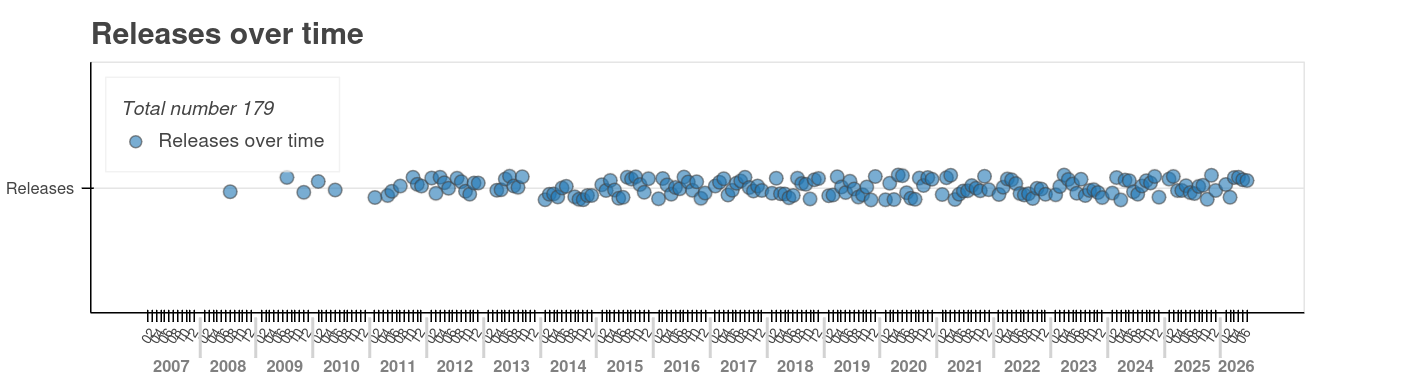
\includegraphics[width=0.99\linewidth]{./img/misp-releases.png}
    \end{center}
\end{frame}

\begin{frame}
    \frametitle{What is MISP?}
    \begin{itemize}
        \item Used worldwide to \textbf{manage and share threat-related information and intelligence}.
        \item \textbf{Open-Source Commitment}: Users of MISP can rely on the tool remaining open source and never becoming closed source (autonomy of the users).
    \end{itemize}

    \begin{center}
        
\includegraphics[width=0.99\linewidth]{./img/contributors.png}
        \vspace{0.1em}
        \scriptsize \texttt{Number recorded on March 2026}
    \end{center}
\end{frame}

\begin{frame}
    \frametitle{What is MISP?}
    \begin{itemize}
        \item A tool that {\bf collects} from partners, your analysts, your tools, feeds, $\cdots$
        \item Normalises, {\bf correlates}, {\bf enriches} the data
        \item Allows teams and communities to {\bf collaborate} and {\bf share}
        \item {\bf Feeds} automated protective tools and {\bf disseminate}
    \end{itemize}
\end{frame}

\begin{frame}
    \frametitle{Who is Using MISP?}
    \vspace{-1em}
    \textbf{Communities:} Groups of users sharing within a set of common objectives and values.
    \vspace{1em}

    \begin{columns}[T]
    \begin{column}{0.5\textwidth}
        \begin{itemize}
            \item \textbf{Private Sector}
                \vspace{-0.2em}
                \begin{itemize}
                    \item[] Financial, telecom, manufacturing
                \end{itemize}
                % \vspace{0.1em}
            \item \textbf{Military Organizations}
                \vspace{-0.2em}
                \begin{itemize}
                    \item[] Military and governmental CERT
                \end{itemize}
                % \vspace{0.1em}
            \item \textbf{Security Vendors}
                \vspace{-0.2em}
                \begin{itemize}
                    \item[] Vendor-led intelligence sharing
                \end{itemize}
                % \vspace{0.1em}
            \item \textbf{ISACs}
            \item \textbf{Trusted Groups}
                \vspace{-0.2em}
                \begin{itemize}
                    \item[] Inc. air-gapped trusted sharing
                \end{itemize}
                % \vspace{0.1em}
            \item \textbf{Law Enforcement Agencies}
            \item \textbf{International Groups}
        \end{itemize}
    \end{column}
    \hfill
    \begin{column}{0.5\textwidth}
        \centering
        \hfil
        
\includegraphics[width=\linewidth, keepaspectratio]{./img/org-count-misppriv.png}
        \vspace{0.1em}
        \scriptsize \texttt{Aggregated from misppriv.circl.lu (June 2026)}
    \end{column}
    \end{columns}

\end{frame}

\begin{frame}
    \frametitle{MISP and Threat Intelligence}
    \vspace{-1em}
    MISP is designed from the ground up to perform \textbf{context-rich threat intelligence}
    \vspace{1em}

    \begin{columns}[T]
    \begin{column}{0.55\textwidth}
        \begin{itemize}
            \item {\bf Enrich} information with context and metadata
            \item Maps {\bf Threats and TTPs}
                \vspace{-0.2em}
                \begin{itemize}
                    \item[] {\small e.g MITRE ATT\&CK}
                \end{itemize}
                \vspace{0.1em}
            \item Supports many {\bf standardized classification} marking
            \item Enables information {\bf curation} through automated quality checks
            \item Generates customizable {\bf threat reports}
            \item Allows creation of {\bf Dashboard} for trend analysis
        \end{itemize}
    \end{column}
    \hfill
    \begin{column}{0.45\textwidth}
        \centering
        \hfil
        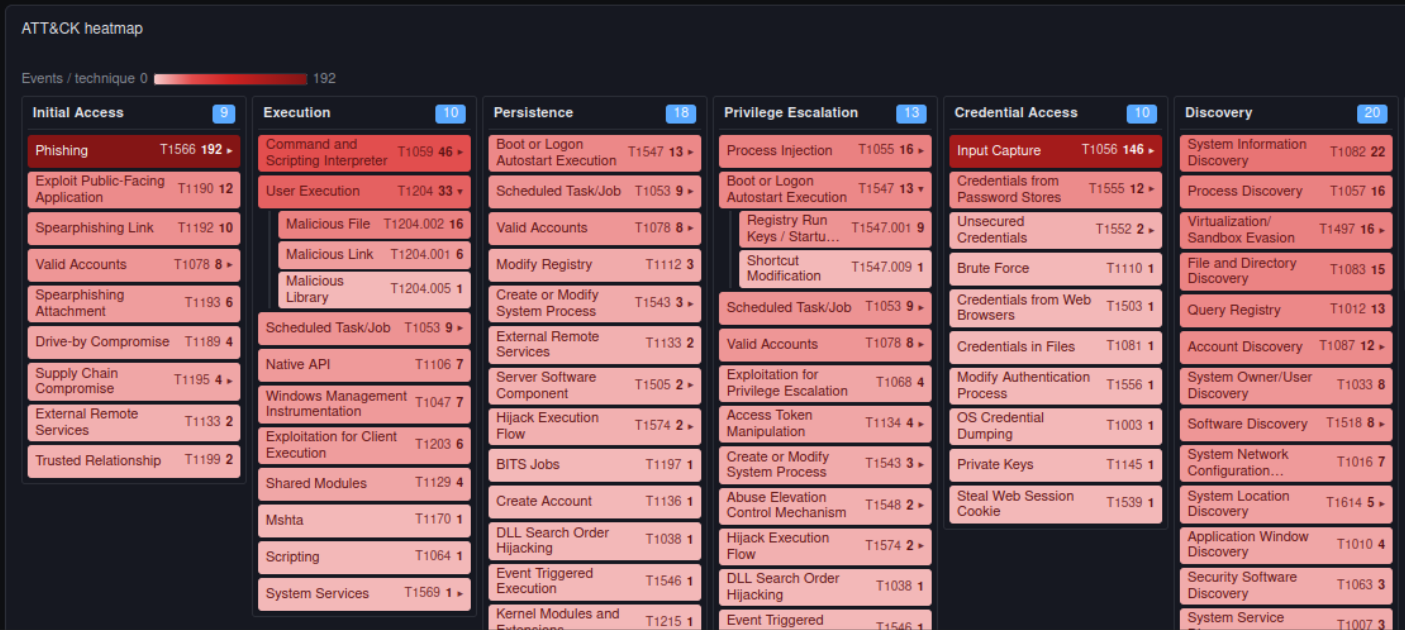
\includegraphics[width=\linewidth, keepaspectratio]{./img/misp-ttps.png}
        \vspace{0.1em}
        \scriptsize \texttt{MITRE ATT\&CK Matrix}
    \end{column}
    \end{columns}
\end{frame}

\begin{frame}
    \frametitle{Information Quality Management}

    MISP provides mechanisms to maintain, enrich and operationalize intelligence throughout its lifecycle.

    \begin{center}
        \begin{columns}[T]
            \begin{column}{0.6\textwidth}
                \card{\linewidth}{1.5em}{\faCheckCircle \, \textbf{Data Quality}}
                    {
                        {\setlength{\leftmargini}{1.0em}
                        \begin{itemize}
                            \item False Positive Management \& Feedback Loops
                            \item Knowledge Base and Vocabularies\\
                                \hspace{1em}{$\triangleright$ \, \small \textit{Address the Who, What, How and Why.}}
                        \end{itemize}
                        }
                    }
            \end{column}
            \hfill
            \begin{column}{0.4\textwidth}
                \card{\linewidth}{1.5em}{\faMagic \, \textbf{Enrichment}}
                    {
                        {\setlength{\leftmargini}{1.0em}
                        \begin{itemize}
                            \item Enrichment system
                            \item Multiple Correlation types\\
                                \hspace{1em}{\small Raw, Fuzzy Hash, CDIR}
                        \end{itemize}
                        }
                    }
            \end{column}
        \end{columns}
        % \vspace{0.5em}
        \begin{columns}[T]
            \begin{column}{0.5\textwidth}
                \card{\linewidth}{1.5em}{\faGavel \, \textbf{Governance}}
                    {
                        {\setlength{\leftmargini}{1.0em}
                        \begin{itemize}
                            \item Review Workflows
                            \item Publication Control
                            \item Lifecycle Management
                        \end{itemize}
                        }
                    }
            \end{column}
            \hfill
            \begin{column}{0.5\textwidth}
                \card{\linewidth}{1.5em}{\faLink \, \textbf{Integration}}
                    {
                        {\setlength{\leftmargini}{1.0em}
                        \begin{itemize}
                            \item API \& Automation ecosystem
                            \item Integration with External Tools
                            \item Notebooks
                        \end{itemize}
                        }
                    }
            \end{column}
        \end{columns}
    \end{center}
\end{frame}

\begin{frame}
    \frametitle{Flexible Data Format}

    \begin{center}
        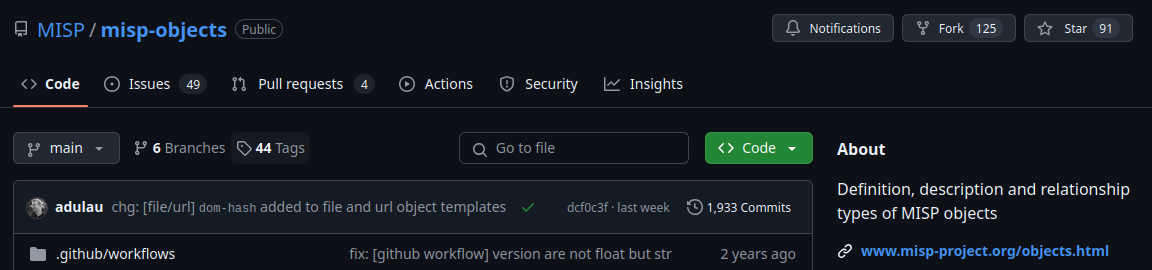
\includegraphics[width=0.8\linewidth]{./img/misp-objects-repo.png}
    \end{center}

    % \vspace{0.3em}
    \begin{center}
        \small
        MISP Objects provide reusable templates to model virtually any investigative artifact.
    \end{center}
    \vspace{0.1em}

    \centering

       \begin{center}
        \begin{columns}[T]
            \begin{column}{0.33\textwidth}
                \card{\linewidth}{1.5em}{\faGlobe \, \textbf{Network}}
                    {IPs, URLs, hashes}
            \end{column}
            \hfill
            \begin{column}{0.33\textwidth}
                \card{\linewidth}{1.5em}{\faLaptop \, \textbf{Devices}}
                    {Phones, software}
            \end{column}
            \begin{column}{0.33\textwidth}
                \card{\linewidth}{1.5em}{\faCreditCard \, \textbf{Payments}}
                    {Cards, transactions, crypto}
            \end{column}
        \end{columns}
        % \vspace{0.5em}
        \begin{columns}[T]
             \begin{column}{0.33\textwidth}
                \card{\linewidth}{1.5em}{\faCar \, \textbf{Vehicles}}
                    {Cars, aircraft, drones}
            \end{column}
            \hfill
            \begin{column}{0.33\textwidth}
                \card{\linewidth}{1.5em}{\faIdCard \, \textbf{Identities}}
                    {Persons, passports, PNR}
            \end{column}
            \begin{column}{0.33\textwidth}
                \card{\linewidth}{1.5em}{\faPuzzlePiece \, \textbf{Extensible...}}
                    {420+ Templates}
            \end{column}
        \end{columns}
    \end{center}

\end{frame}

\begin{frame}
    \frametitle{Rich Marking and Knowledge Base}

    \begin{columns}[T,onlytextwidth]
        \column{0.5\textwidth}
        \begin{itemize}
            \item \textbf{Typical CTI}
            \begin{itemize}
                \item Threat Actors
                \item Countries
                \item Attack Techniques
                \item Campaigns
                \item And \textbf{many more} $\cdots$
            \end{itemize}
        \end{itemize}

        \vspace{0.5em}

        \begin{itemize}
            \item \textbf{Impact}
            \begin{itemize}
                \item Geographical / Sectorial
                \item Demographical
                \item Economical / Legal / Regulatory
                \item Assets / Users
                \item Affected availabilities / Data Integrity
            \end{itemize}
        \end{itemize}

        \column{0.5\textwidth}

        \begin{itemize}
            \item \textbf{Confidentiality}
            \begin{itemize}
                \item Copyrighted / Classified
                \item Disclosure
            \end{itemize}
        \end{itemize}

        \vspace{0.5em}

        \begin{itemize}
            \item \textbf{Responsibility}
            \begin{itemize}
                \item Governance - 3rd party Hosted
                \item Management / Ownership
                \item Confidence / Estimative Language
                \item Discovery
            \end{itemize}
        \end{itemize}

        \vspace{0.5em}

        \begin{itemize}
            \item \textbf{Extensible} $\cdots$
            \begin{itemize}
                \item {350+ Different Vocabularies}
            \end{itemize}
        \end{itemize}

    \end{columns}
\end{frame}


\begin{frame}
    \frametitle{Using the Power of the Community}

    MISP provides multiple mechanisms to foster collaboration between analysts, teams and communities.

    % \vspace{1em}

    \begin{center}

        \begin{columns}[T]

            \begin{column}{0.49\textwidth}
                \card{\linewidth}{2.5em}
                    {{\Large\faUsers}\hspace{0.3em}\textbf{Collaboration}}
                    {
                        \begin{itemize}
                            \item Proposals
                            \item Sightings
                            \item Extended Events
                        \end{itemize}
                    }
            \end{column}

            \begin{column}{0.49\textwidth}
                \card{\linewidth}{2.5em}
                    {{\Large\faComments}\hspace{0.3em}\textbf{Discussion}}
                    {
                        \begin{itemize}
                            \item Analyst Notes
                            \item Opinions
                        \end{itemize}
                    }
            \end{column}

        \end{columns}

        \vspace{-0.5em}
        \centering
        \begin{columns}[T]

            \begin{column}{0.6\textwidth}
            \card{1.0\linewidth}{2.5em}
                {{\Large\faGlobe}\hspace{0.3em}\textbf{Specialized Sharing}}
                {
                    \begin{itemize}
                        \item Delegation
                        \item Sharing Groups
                        \item Trust Communities
                    \end{itemize}
                }
                \end{column}

        \end{columns}
    \end{center}

    \vspace{1em}

    \centering
    \small
    Collaboration can happen within a team, across organizations, or through trusted sharing communities.

\end{frame}



% =========================================================
% New Features
% =========================================================
\storyphase{New Features}

\nosectionpage{New features in the past few months}
\subsection{MISP Highlights}

\begin{frame}
  \frametitle{New features in the past few months - June 2026}

    \vspace{-2em}


    \begin{center}
    \begin{tikzpicture}[
        stat/.style={
            draw,
            rounded corners,
            minimum width=3.2cm,
            minimum height=1.8cm,
            align=center,
            fill=structure.fg,
            text=white
        },
    ]

    \node[stat] (r1) {
        {\Huge\bfseries 16}\\[-0.2em]
        {\scriptsize Releases}
    };

    \node[stat, right=0.5cm of r1] (r2) {
        {\Huge\bfseries 2851}\\[-0.2em]
        {\scriptsize Total Commits}
    };

    \node[stat, right=0.5cm of r2] (r3) {
        {\Huge\bfseries 167}\\[-0.2em]
        {\scriptsize Pull Requests}
    };

    \node[stat, right=0.5cm of r3] (r4) {
        {\Huge\bfseries 72}\\[-0.2em]
        {\scriptsize Contributors}
    };

    \end{tikzpicture}

    \vspace{1.0em}

    \begin{tikzpicture}[
        stat/.style={
            draw,
            rounded corners,
            minimum width=3.2cm,
            minimum height=1.8cm,
            align=center,
            fill=structure.fg,
            text=white
        }
    ]

    \node[
        draw,
        rounded corners,
        minimum width=14.4cm,
        minimum height=1.2cm,
        align=center,
        fill=structure.fg,
        text=white
    ] (detail) {
        \small
        \textbf{1619} commits on MISP core
        \hspace{1em}$\bullet$\hspace{1em}
        \textbf{1232} commits across 18 modules
        \hspace{1em}$\bullet$\hspace{1em}
        \textbf{145} merged pull requests
    };

    \end{tikzpicture}
    \end{center}

    % \vspace{1.0em}

    \begin{itemize}
        \item {\bf UI/UX modernisation}
        \item New {\bf dashboard} system
        \item New {\bf event templating} system
        \item {\bf Geolocation \& map} visualisation
        \item \textbf{Continuous Security Hardening} --- \alert{Regular updates remain critical}
    \end{itemize}

\end{frame}


\begin{frame}
    \frametitle{UI/UX modernisation}

    \vspace{-4em}
    \alertbox{info}{The biggest visual change in years!}{}
    \vspace{-0.3em}

    \begin{itemize}
        \item {\bf Theme system} --- opt-in themes let users preview new UIs
        \begin{itemize}
            \item {\bf BetaUI} --- a community-contributed UX rework (Chris Horsley, Cosive)
                \begin{itemize}
                    \item[] A redesigned, responsive event index \& reorganised navigation
                \end{itemize}
            \item {\bf Overmind} --- the next-generation interface
                \begin{itemize}
                    \item[] Refreshed look and new views
                \end{itemize}
        \end{itemize}
        \item {\bf Decomposed event view} --- the monolithic event view split into specialized views
        \item {\bf Modern front-end stack} Migrating MISP to {\bf Bootstrap 5} and {\bf Font Awesome 7}
    \end{itemize}

\end{frame}

\begin{frame}
    \frametitle{UI/UX modernisation}

    \begin{center}

    \begin{minipage}[t]{0.43\textwidth}
        \centering
        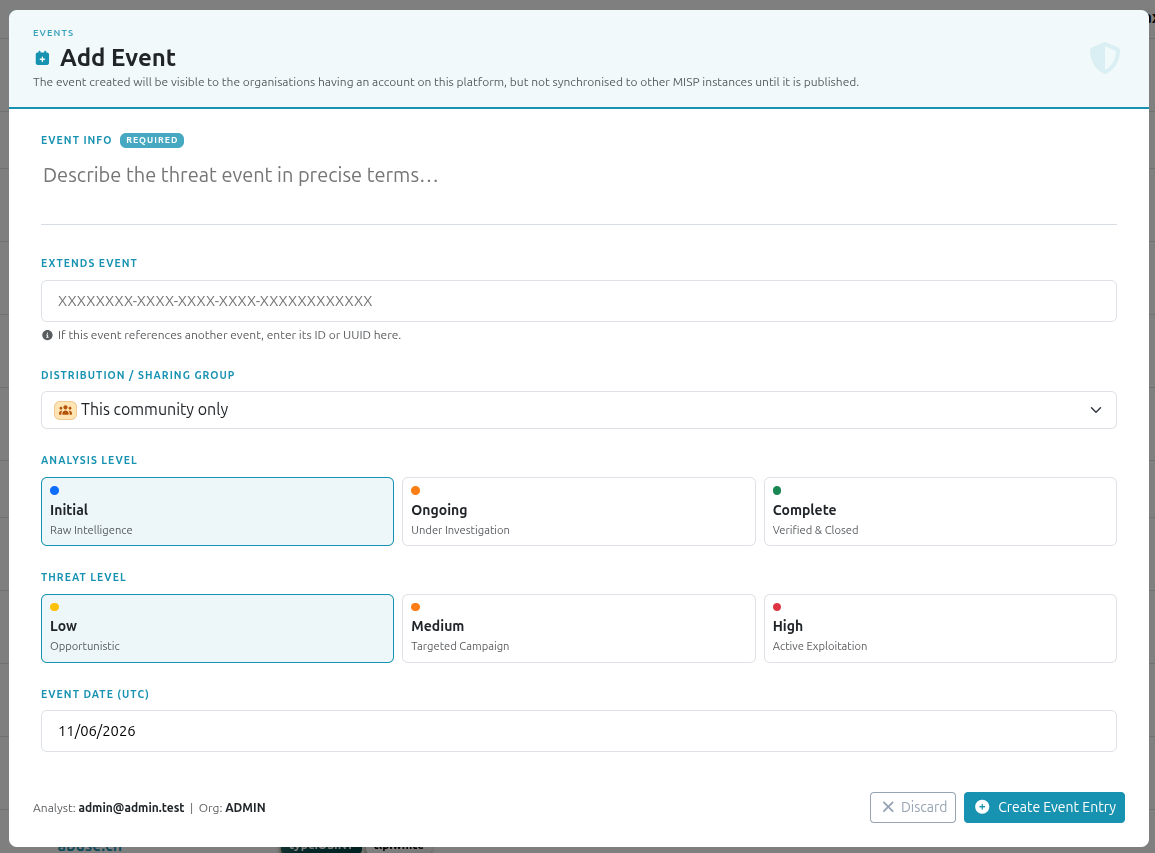
\includegraphics[width=\linewidth, height=0.32\textheight, keepaspectratio]{./img/event-add}

        \vspace{0.3em}
        \scriptsize \texttt{/event/add}
    \end{minipage}
    \hfill
    \begin{minipage}[t]{0.55\textwidth}
        \centering
        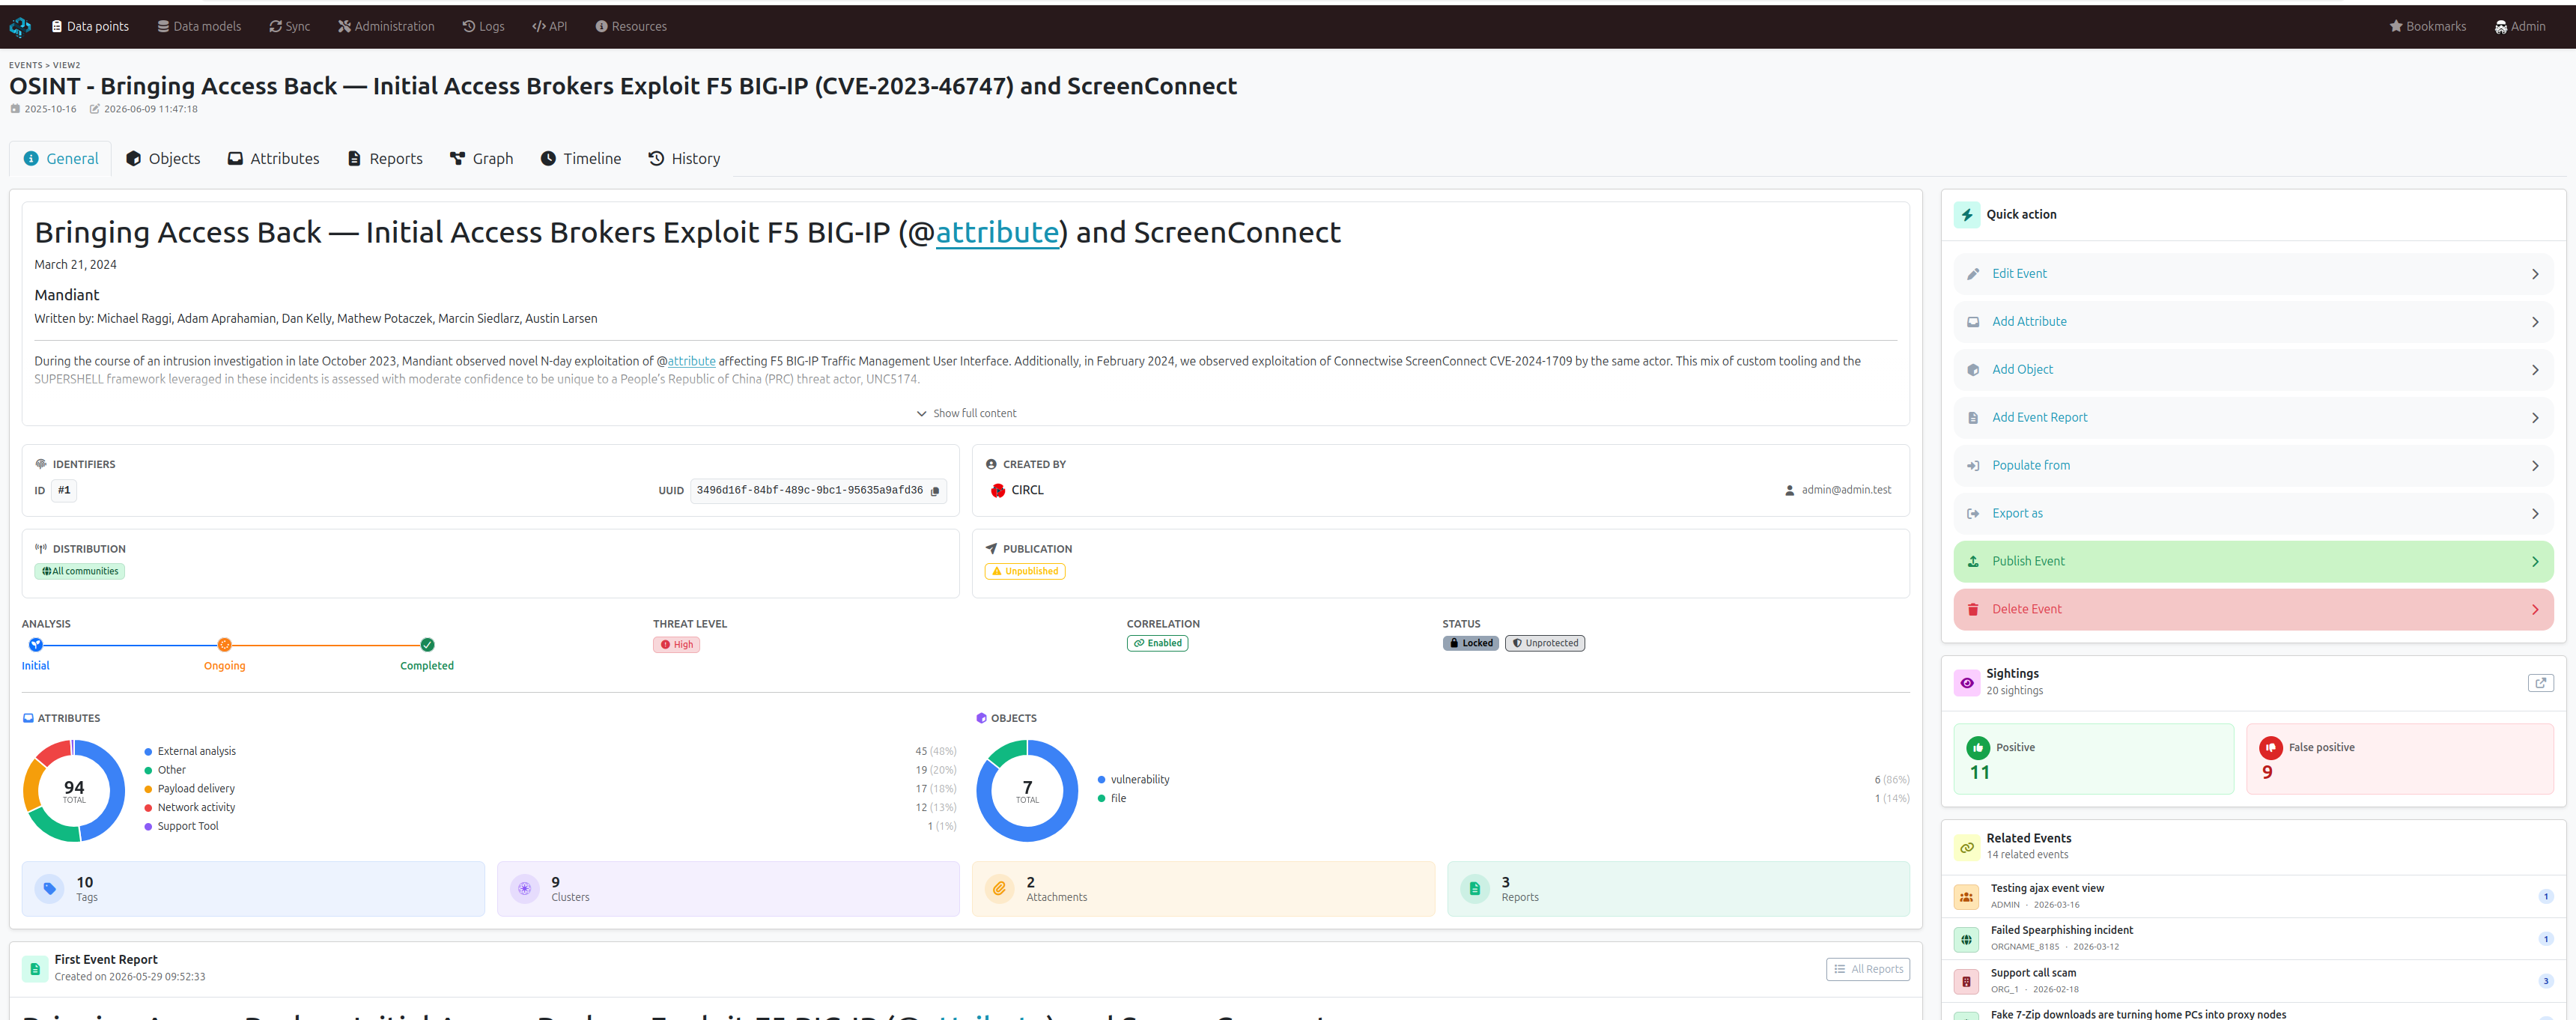
\includegraphics[width=\linewidth, height=0.32\textheight, keepaspectratio]{./img/event-overmind}

        \vspace{0.1em}
        \scriptsize \texttt{/event/view}
    \end{minipage}

    \vspace{0.5em}

    \begin{minipage}[t]{0.48\textwidth}
        \centering
        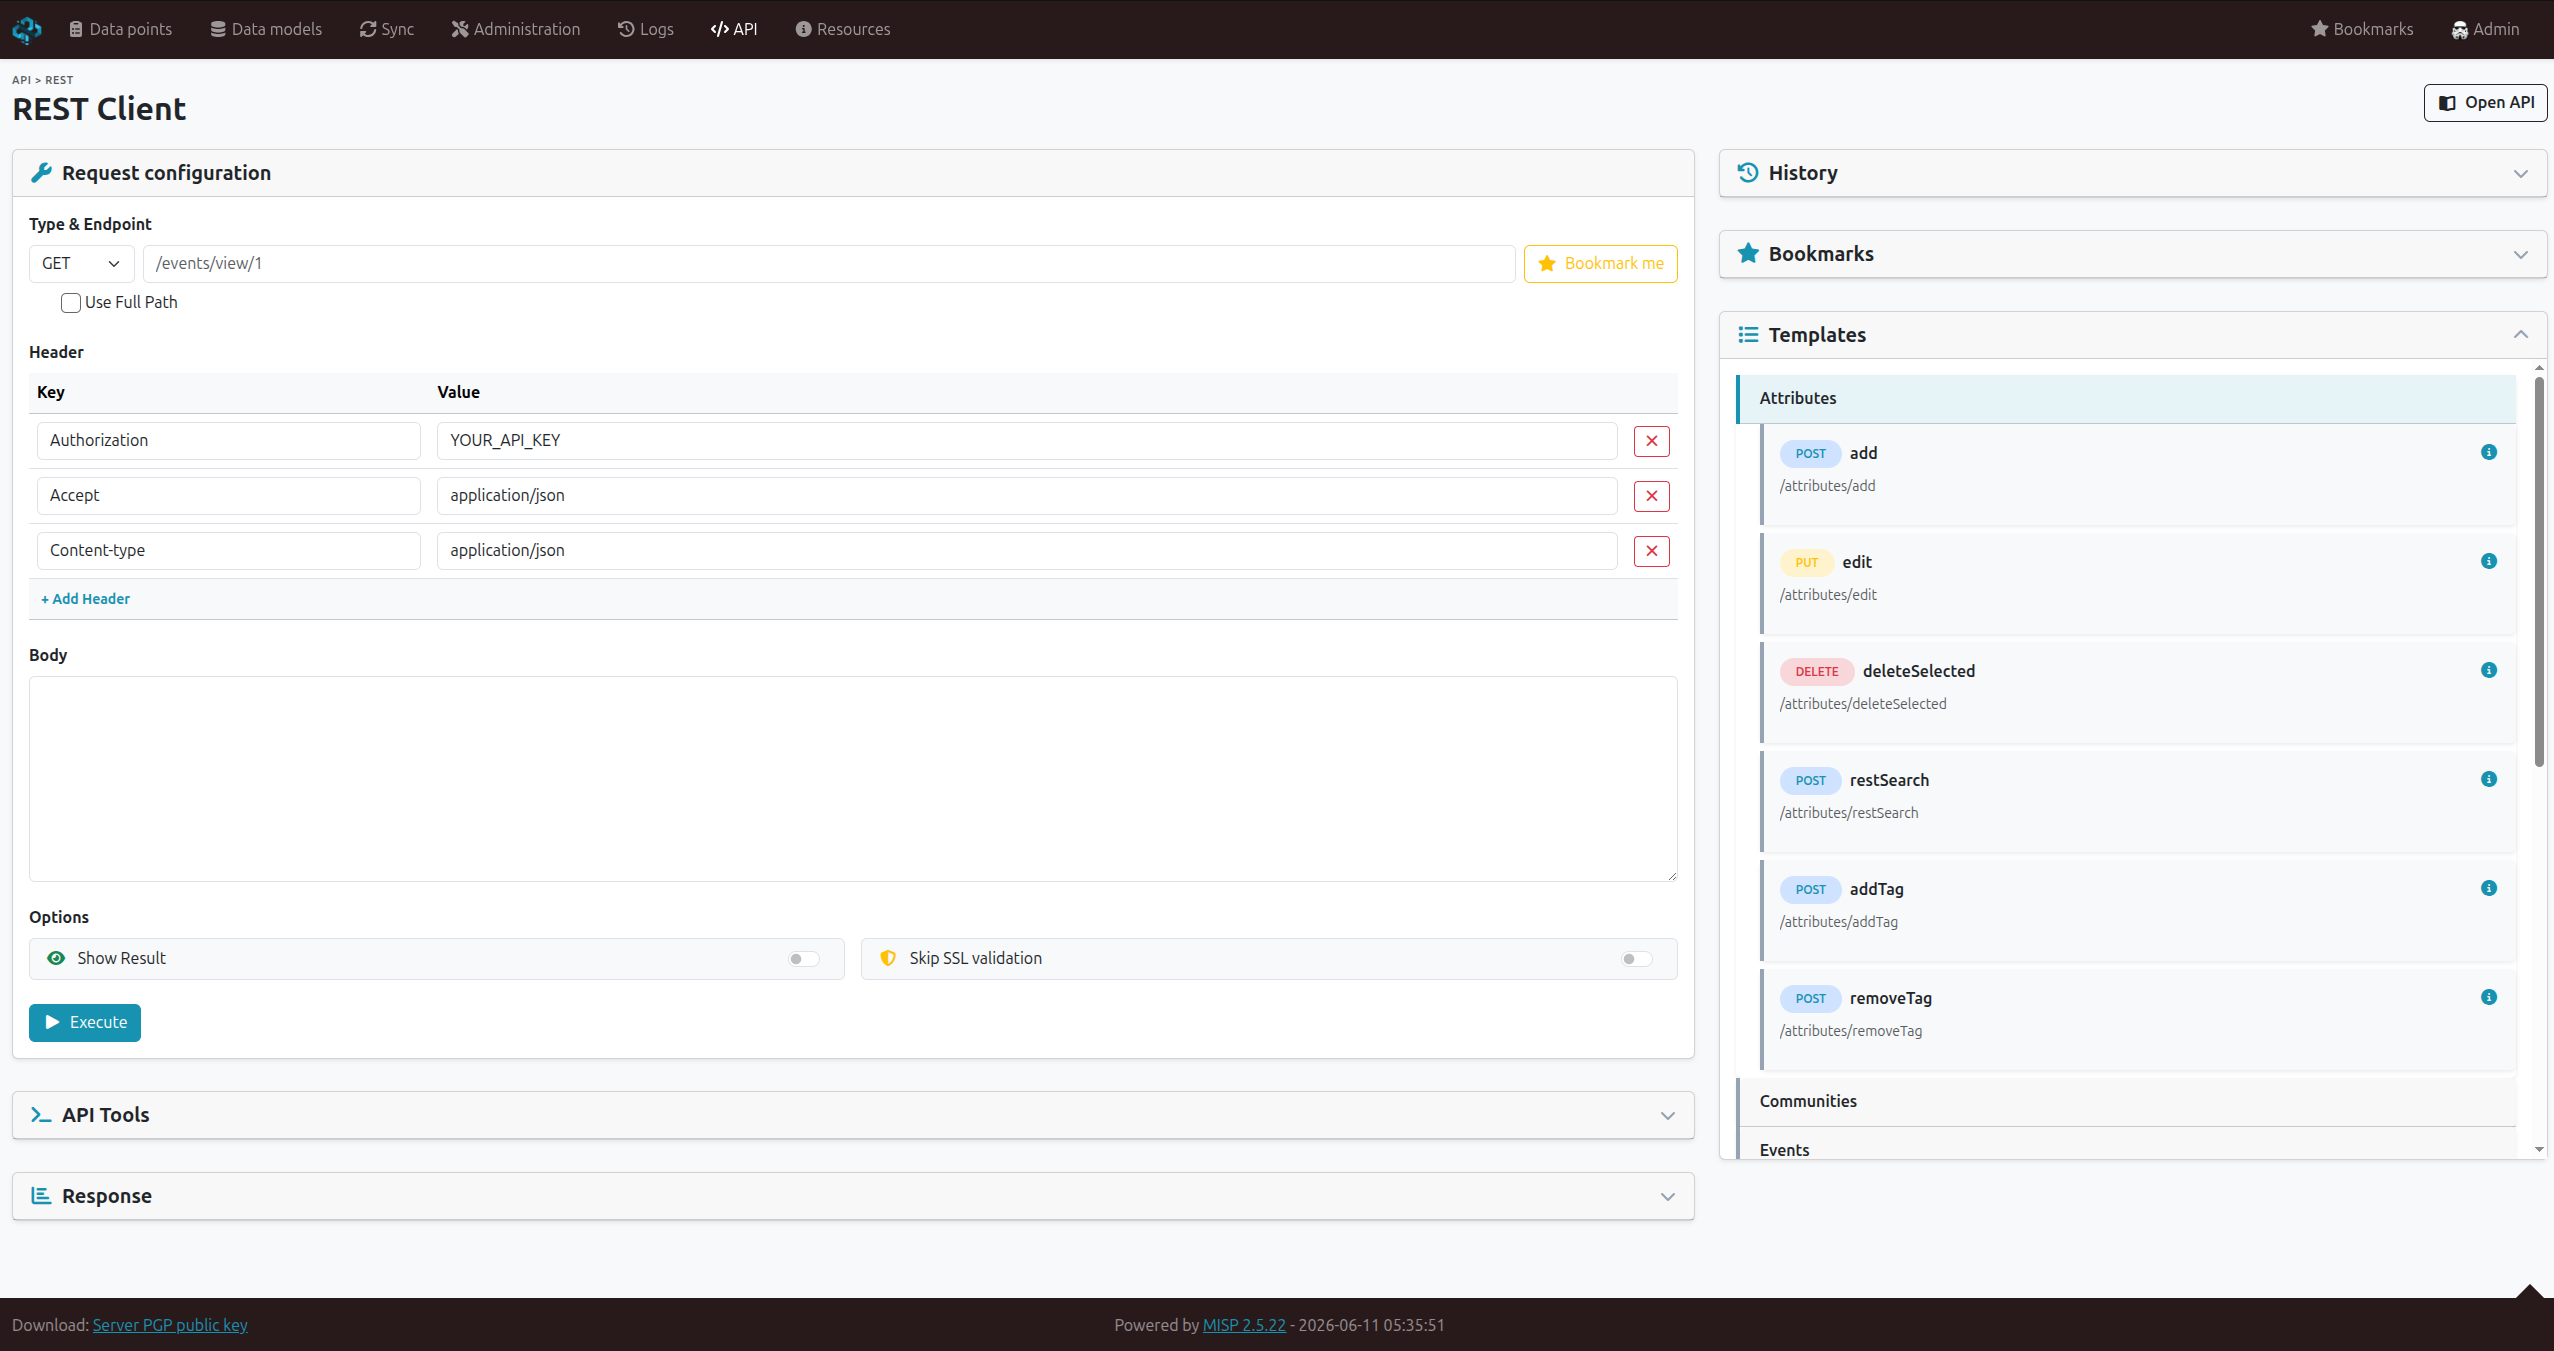
\includegraphics[width=\linewidth, height=0.32\textheight, keepaspectratio]{./img/rest-client.png}

        \vspace{0.3em}
        \scriptsize \texttt{/api/rest}
    \end{minipage}
    \hfill
    \begin{minipage}[t]{0.48\textwidth}
        \centering
        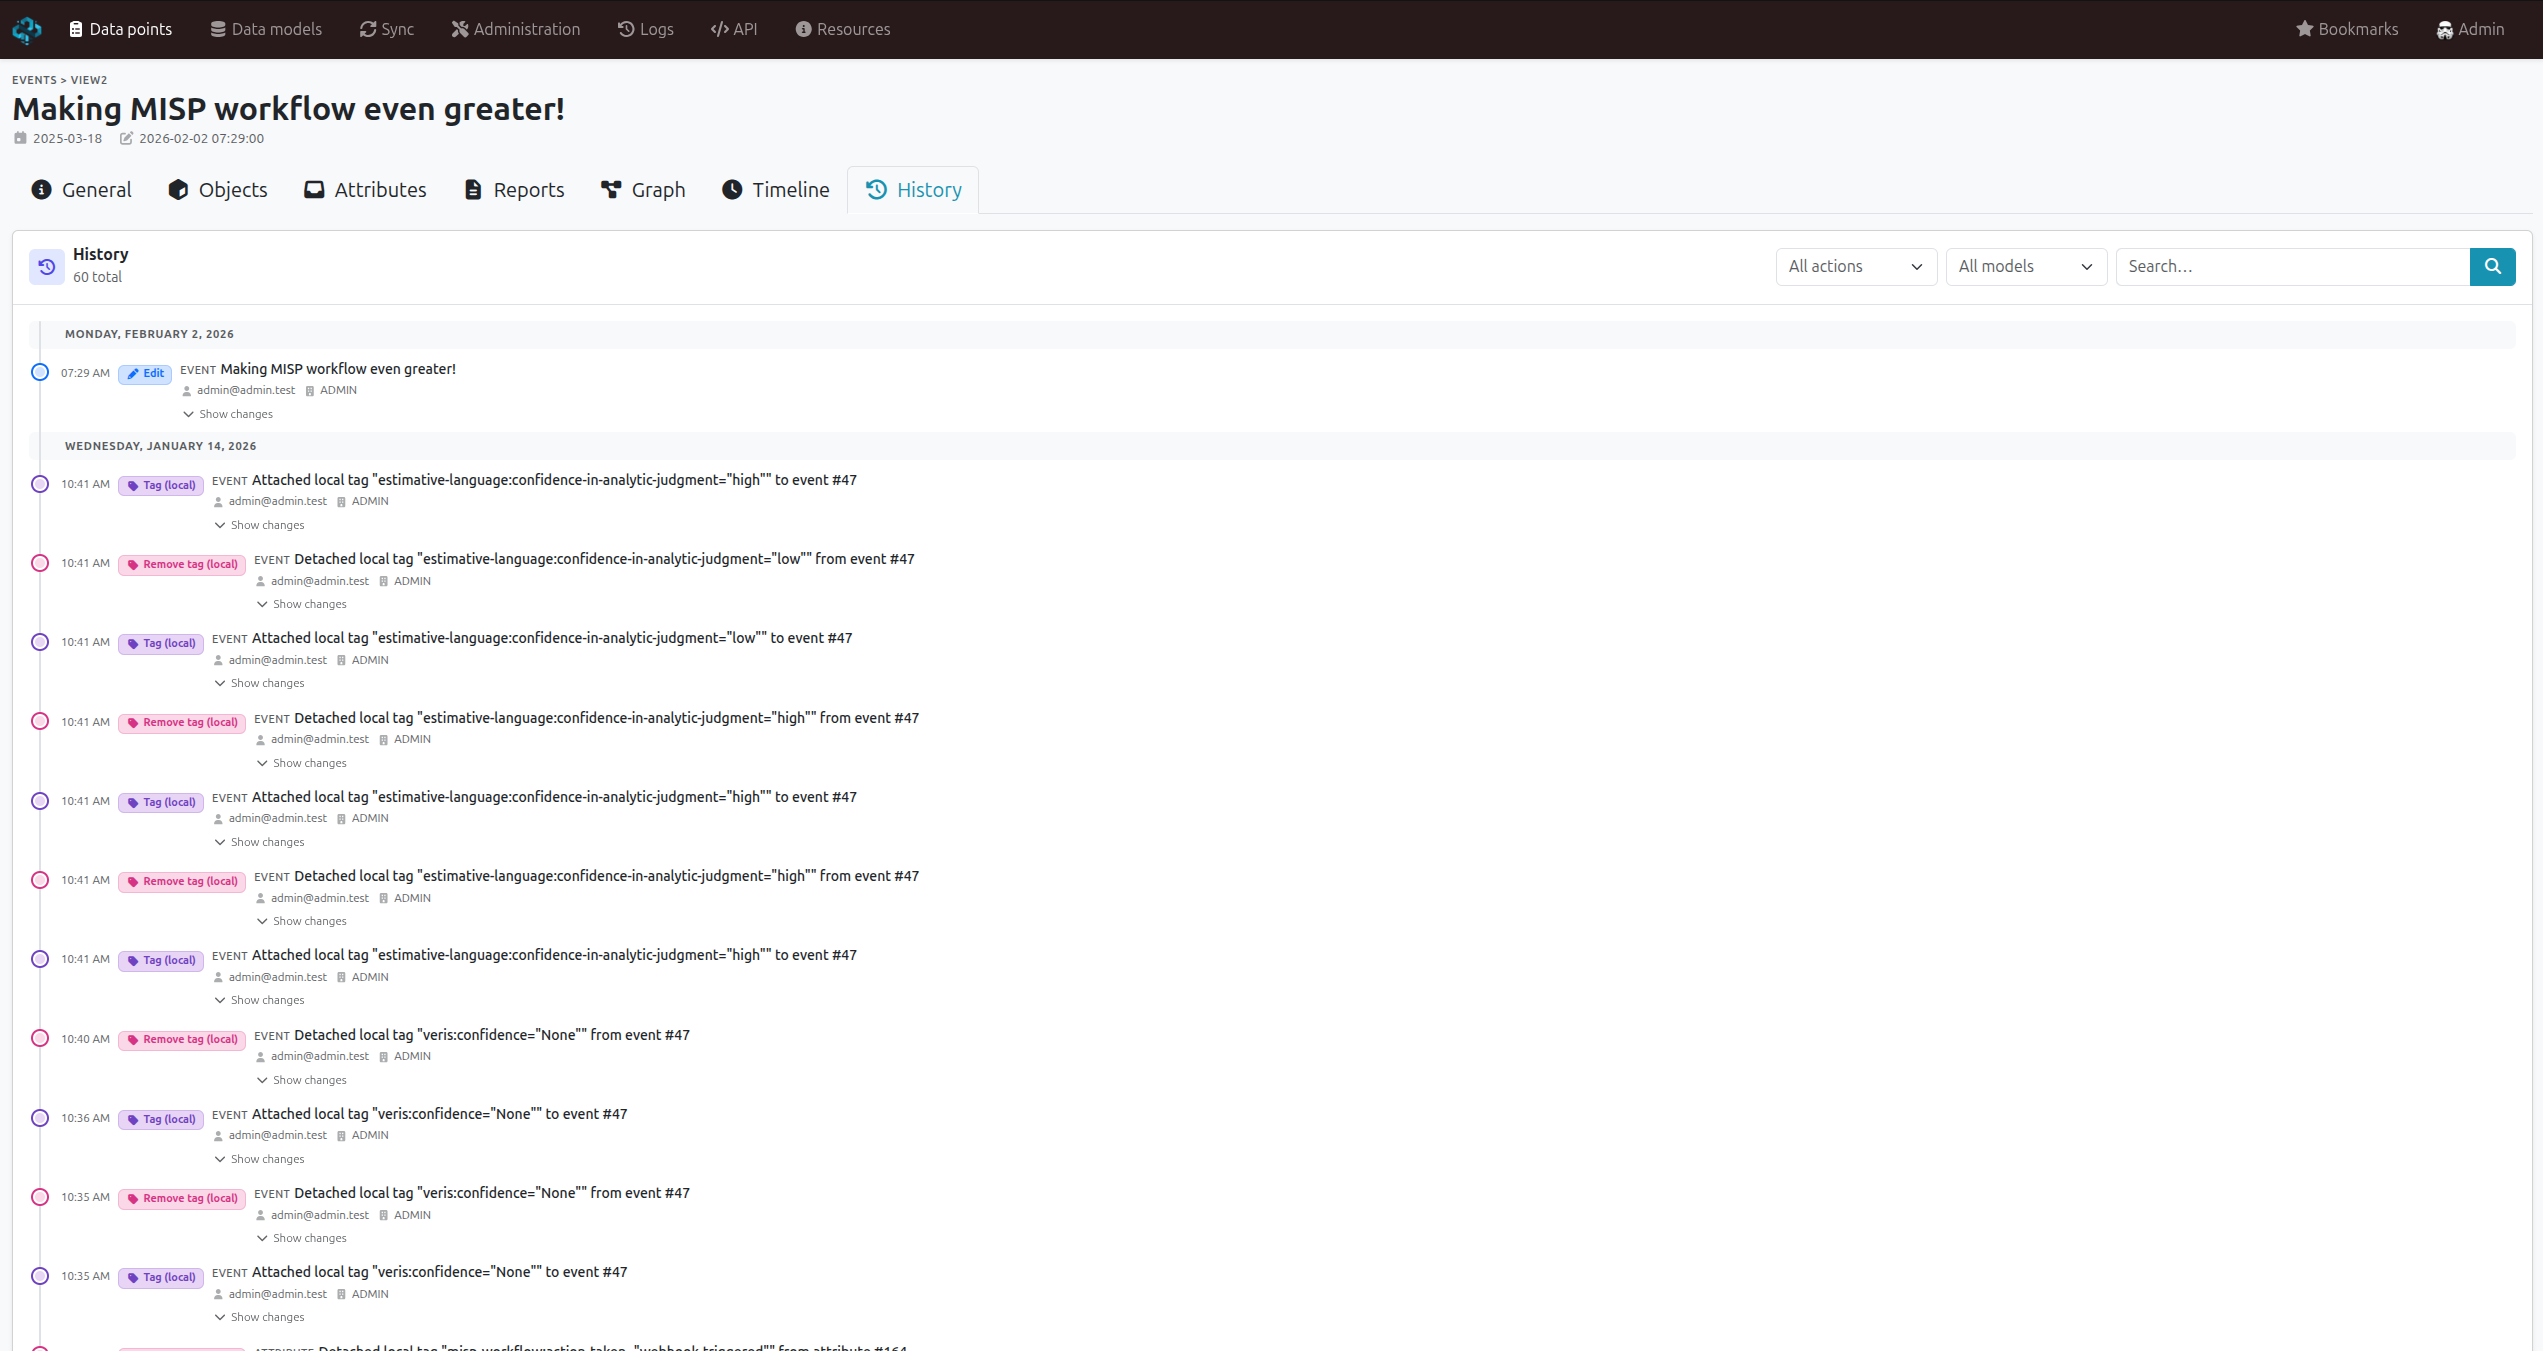
\includegraphics[width=\linewidth, height=0.32\textheight, keepaspectratio]{./img/event-view-history.png}

        \vspace{0.3em}
        \scriptsize \texttt{/event/view-history}
    \end{minipage}

    \end{center}

\end{frame}


\begin{frame}
    \frametitle{New dashboard system}

    \begin{itemize}
        \item A redesign of the MISP dashboard
        \item {\bf Widget gallery} for discovering and adding widgets, with on-demand thumbnails
        \item Richer {\bf chart-based widgets}
        \item Full UI support of parameters and {\bf global dashboard filters}
        \item Foundation for {\bf analyst-focused dashboards} and per-organisation views
    \end{itemize}

\end{frame}


\begin{frame}
    \frametitle{New dashboard system}

    \centering
    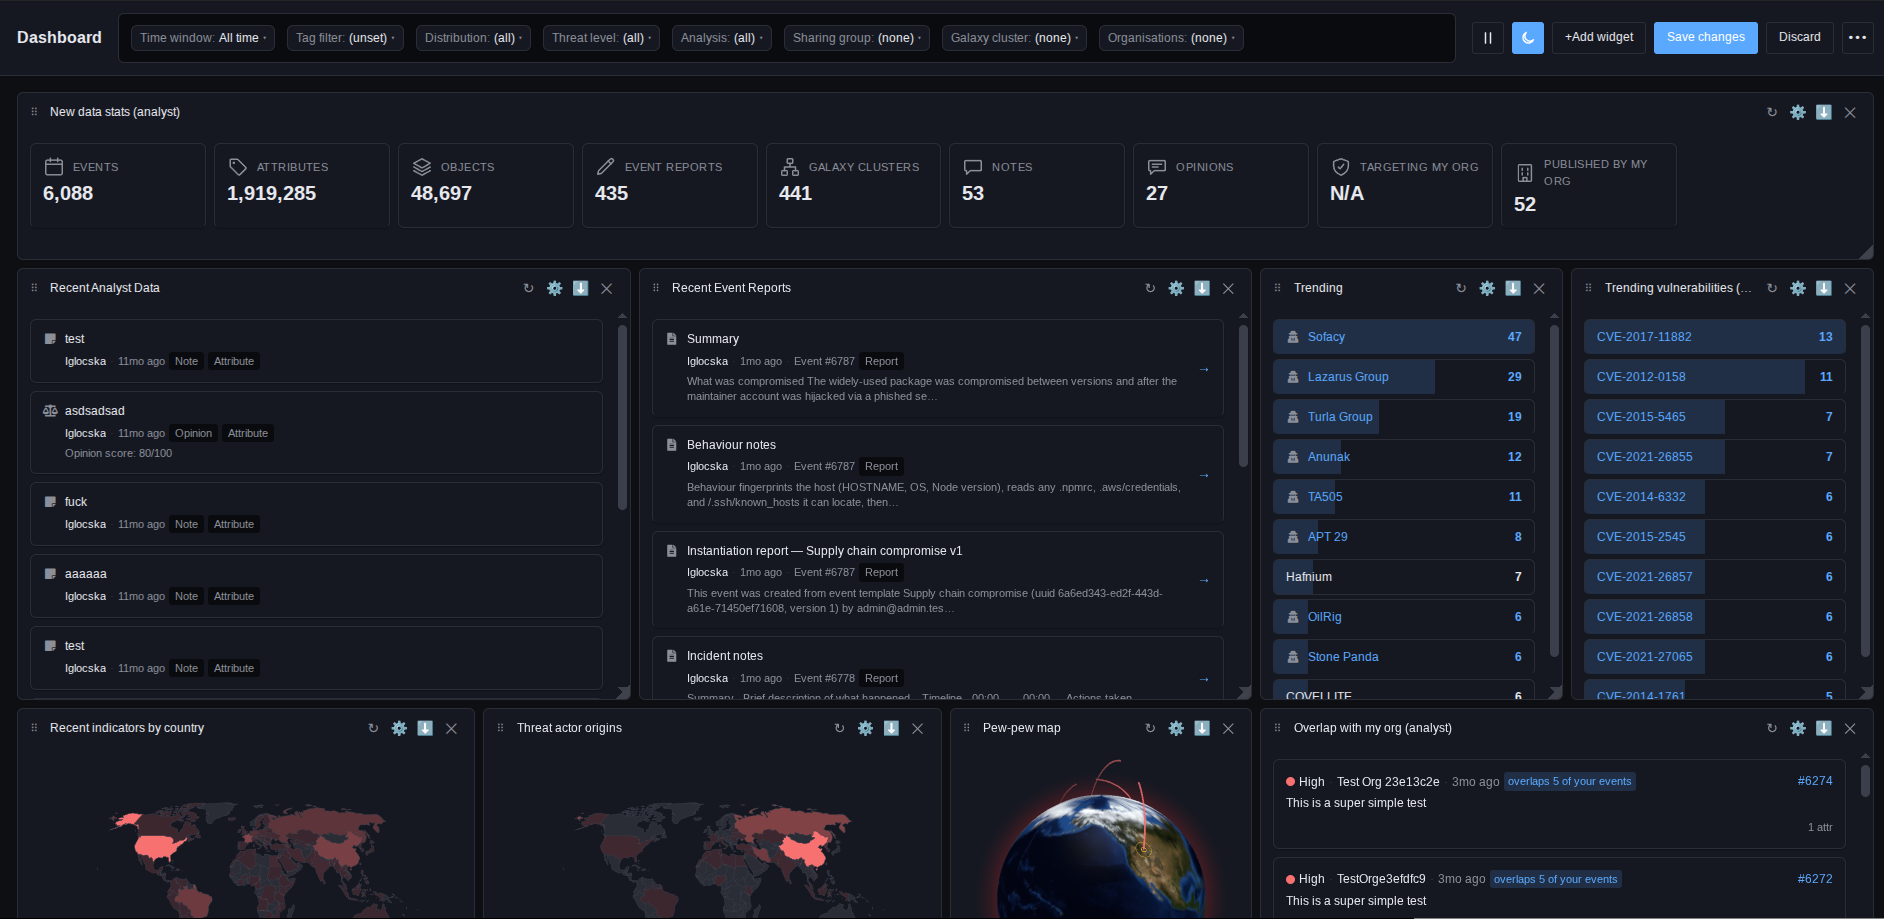
\includegraphics[width=\linewidth, keepaspectratio]{./img/misp-dashboard.png}

\end{frame}

\begin{frame}
    \frametitle{Event templating system}

    \begin{itemize}
        \item A {\bf total rewrite} of MISP's templating engine
        \item {\bf Drag-and-drop builder UI} with inline validation, object-template / taxonomy / galaxy pickers, and a live preview
        \item A {\bf Templates library} ships ten ready-to-use starter templates (ransomware, credential exposure, spearphishing, supply-chain, \dots)
        \item Migration helper for legacy templates, and full documentation
    \end{itemize}

\end{frame}

\begin{frame}
    \frametitle{New dashboard system: Templates Library \& Migration helper}
    \centering
    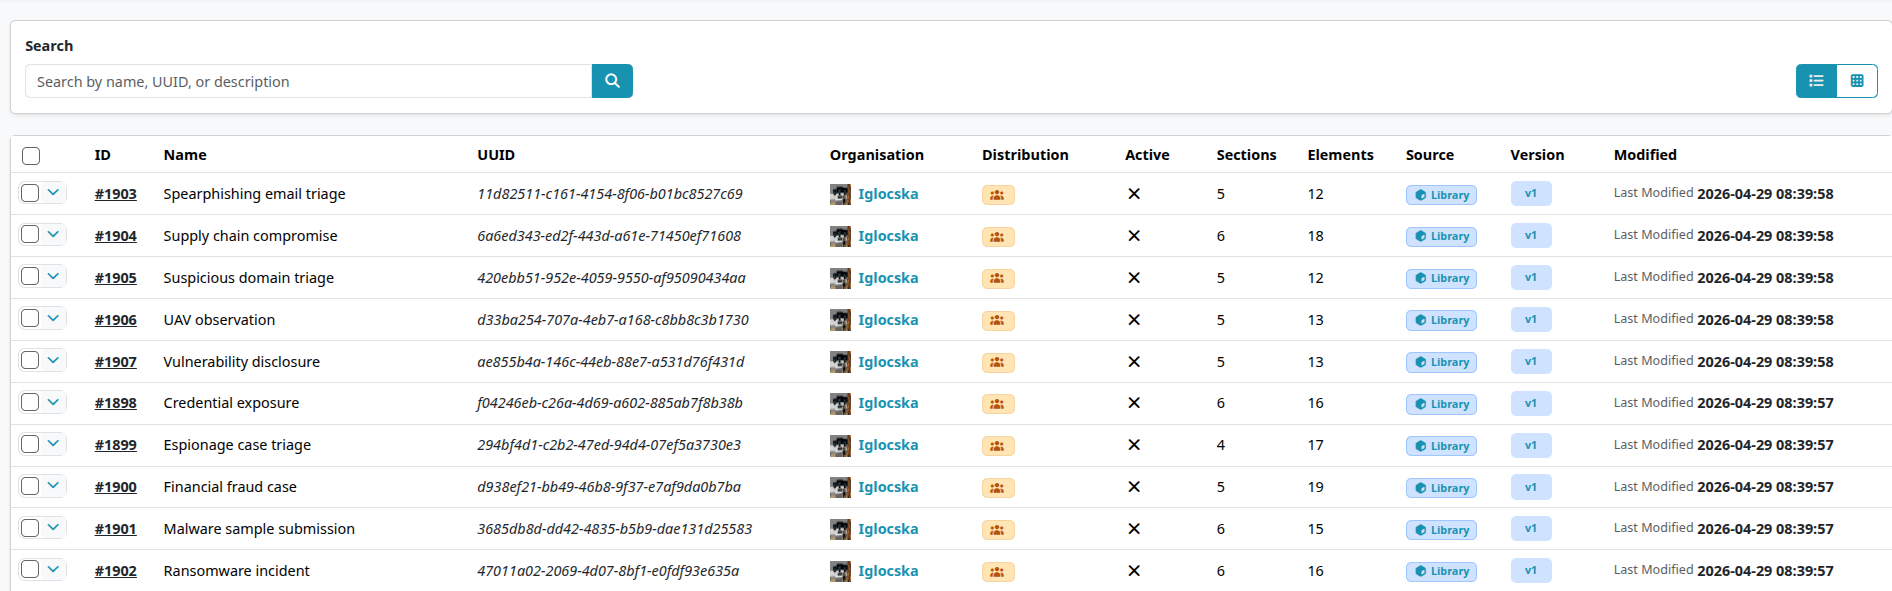
\includegraphics[width=1.0\linewidth, keepaspectratio]{./img/template-index.png}
\end{frame}

\begin{frame}
    \frametitle{New dashboard system: User form}
    \hspace*{-40pt}
    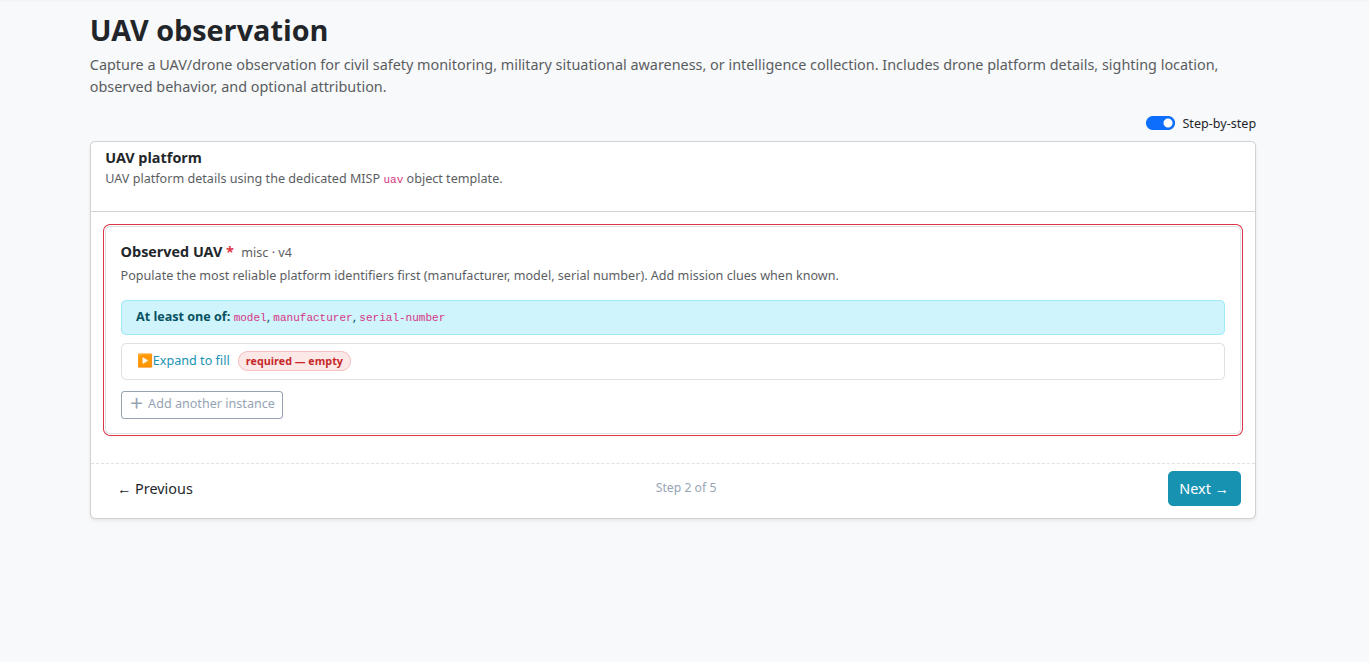
\includegraphics[width=1.2\linewidth, keepaspectratio]{./img/template-use.png}
\end{frame}

\begin{frame}
    \frametitle{New dashboard system: Builder UI}
    \centering
    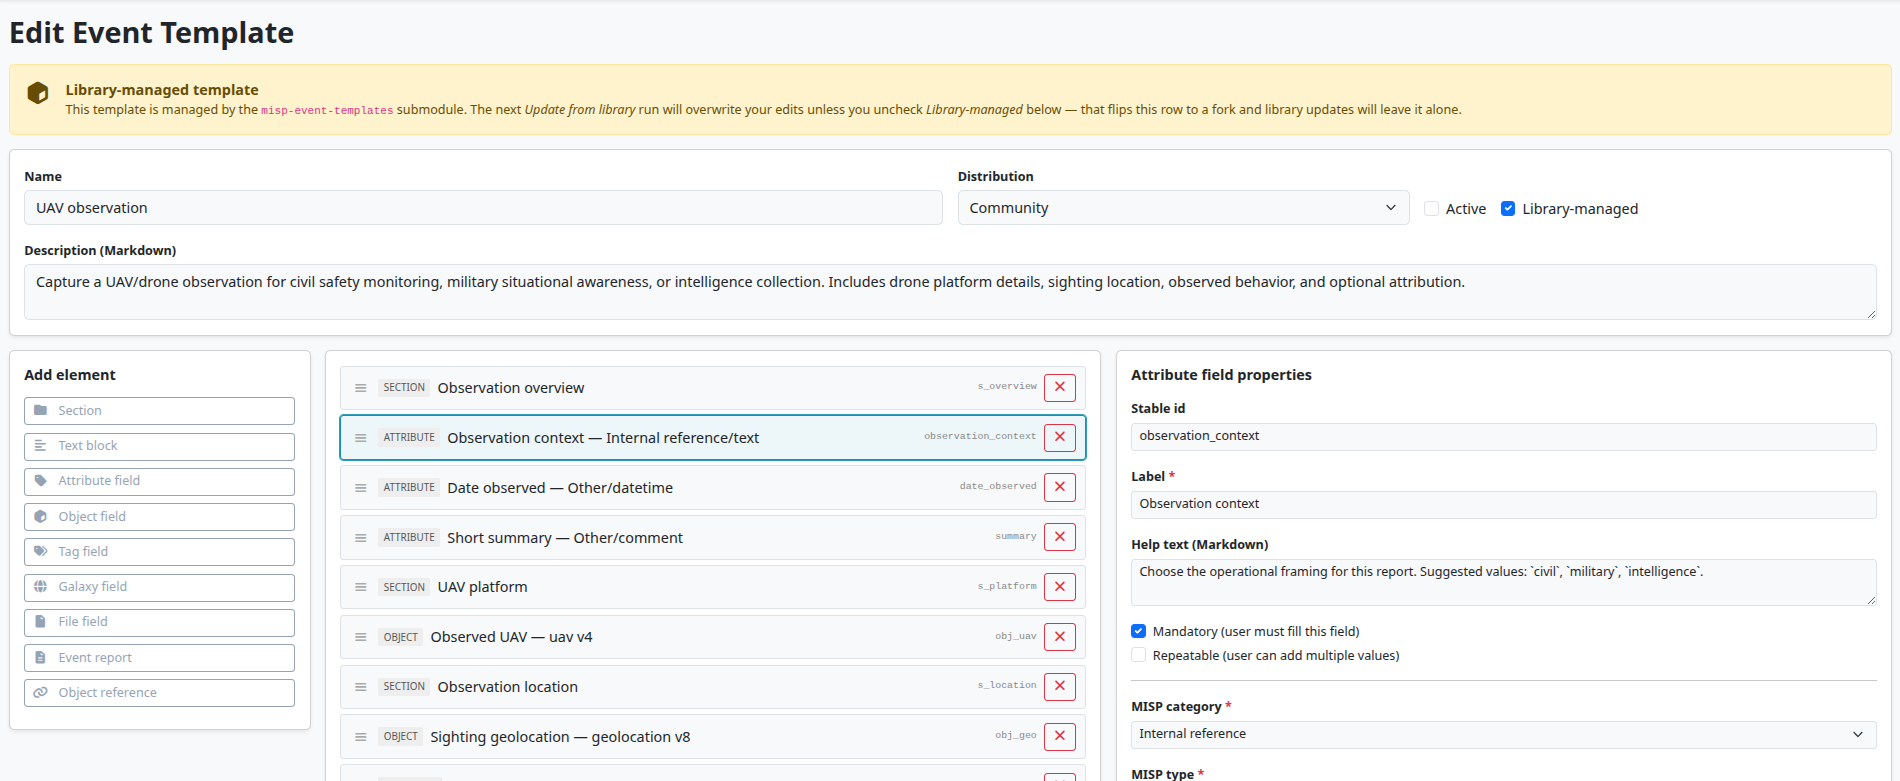
\includegraphics[width=1.0\linewidth, keepaspectratio]{./img/template-edit.png}
\end{frame}

\begin{frame}
    \frametitle{Geolocation \& map visualisation}

    \begin{itemize}
        \item Objects with geographic coordinates are now rendered on {\bf interactive tile-based maps}
        \item {\bf Accuracy-radius} visualisation
        \item Native {\bf GeoJSON} rendering for complex shapes and features
        \item {\bf GPX track} support for tracking objects
    \end{itemize}

    \alertbox{warning}{Disabled by default}{configurable tile server (defaults to \texttt{geo.circl.lu})}
\end{frame}

\begin{frame}
    \frametitle{Geolocation \& map visualisation}

    \begin{center}

    \begin{minipage}[t]{0.48\textwidth}
        \centering
        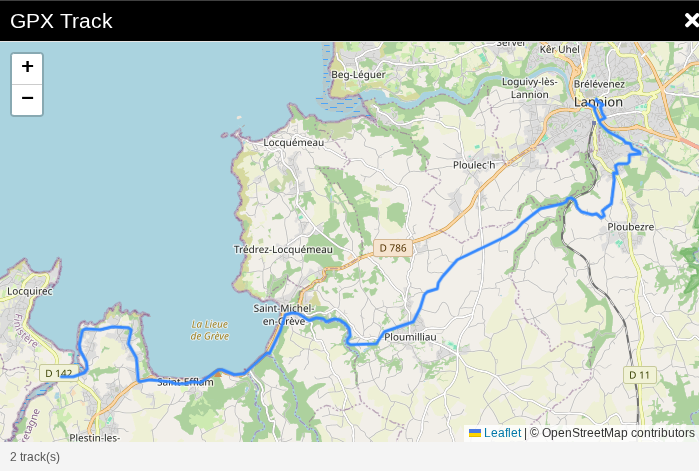
\includegraphics[width=\linewidth, keepaspectratio]{./img/gpx.png}

        \vspace{0.3em}
        \scriptsize \texttt{Full track}
    \end{minipage}
    \hfill
    \begin{minipage}[t]{0.48\textwidth}
        \centering
        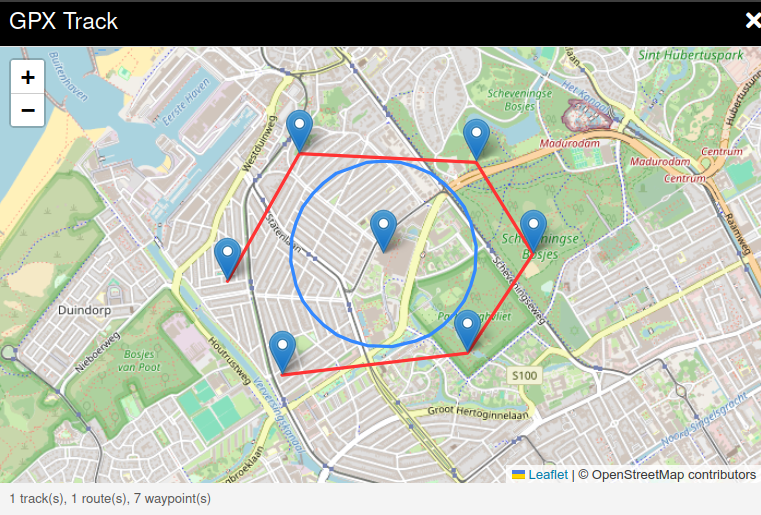
\includegraphics[width=\linewidth, keepaspectratio]{./img/gpx-europol.png}

        \vspace{0.1em}
        \scriptsize \texttt{Routes and waypoints}
    \end{minipage}

    \end{center}
\end{frame}


\end{document}
